%%%%%%%%%%%%%%%%%%%%%%%%%%%%%%%%%%%%%%%%%%%%%%%%%%%%%%%%%%%%%%%%%%%%%%%%
\begin{frame}[t]{[UF95, FL/FR/TL/TR] High Resolution}
\begin{tiny}
\begin{tabular}{@{}lccc@{}}
\toprule
Function & Off/On & Option & Specification \\
\midrule
Audio EQ & \color{blue}{On} & Instart &
\multirow{10}{60mm}{
\begin{itemize}
\item Impulse Response Check
  \begin{itemize}
  \item max impulse를 ref로 정의 (시간: 0s, 크기: 1.0)
  \item 8.5±1ms구간의 max impulse가 ref대비 0.07±0.03 이내
  \item 11.5±1ms구간의 max impulse가 ref대비 0.07±0.03 이내
  \item 14.5±1ms구간의 max impulse가 ref대비 0.07±0.03 이내
  \item 18.5±1ms구간의 max impulse가 ref대비 0.07±0.03 이내
  \item 주요한 impulse는 위의 5구간에서 나타나며, 20ms 이후의 impulse는 분석하지 않음
  \item Left/Right의 3rd, 4th impulse는 허용오차 범위내에서 측정 결과가 다름
  \item AMP와 AP의 연결방법에 의하여 y축 대칭의 결과가 발생
  \end{itemize}
\end{itemize}
} \\
Sound Engine & \color{blue}{On} & Instart & \\
Clearvoice & \color{black}{Off} & & \\
Autovolume & \color{black}{Off} & & \\
Surround & \color{black}{Off} & & \\
Smart Sound & \color{black}{Off} & & \\
3D Sound Zooming & \color{black}{Off} & & \\
Sound Mode & \color{blue}{On} & \color{black}{Standard} & \\
Sound Optimizer & \color{black}{Off} & & \\
OSD Volume & \color{blue}{On} & Vol.40 & \\
 & & & \\
 & & & \\
\midrule
\end{tabular}
\end{tiny}

\begin{figure}[b]
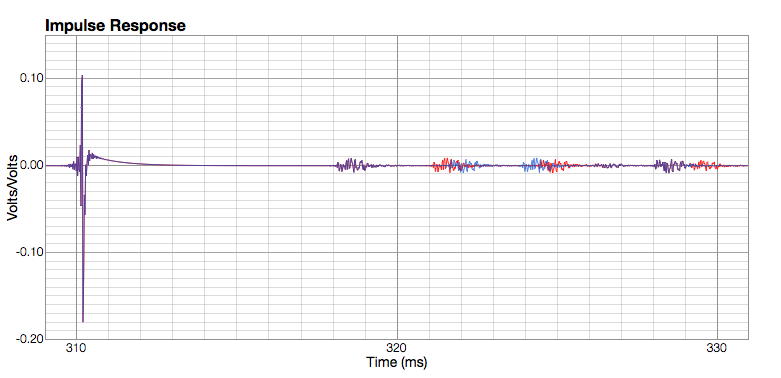
\includegraphics[height=0.4\textwidth]{figures/highresolution.png}
\end{figure}

\end{frame}


